 % !TEX encoding = UTF-8 Unicode
\documentclass[a4paper]{article}

\usepackage{color}
\usepackage{url}
\usepackage[T2A]{fontenc} % enable Cyrillic fonts
\usepackage[utf8]{inputenc} % make weird characters work
\usepackage{graphicx}
\usepackage{float}

\usepackage[english]{babel}
%\usepackage[english,serbian]{babel}
%\usepackage[english,serbianc]{babel} %ukljuciti babel sa ovim opcijama, umesto gornjim, ukoliko se koristi cirilica

\usepackage[unicode]{hyperref}
\hypersetup{colorlinks,citecolor=green,filecolor=green,linkcolor=blue,urlcolor=blue}

\usepackage{listings}

%\newtheorem{primer}{Пример}[section] %ćirilični primer
\newtheorem{primer}{Primer}[section]

\definecolor{mygreen}{rgb}{0,0.6,0}
\definecolor{mygray}{rgb}{0.5,0.5,0.5}
\definecolor{mymauve}{rgb}{0.58,0,0.82}
\definecolor{lightblue}{rgb}{0.67, 0.84, 1}
\definecolor{lightgrey}{rgb}{0.90, 0.90, 0.90}
\definecolor{yelloworange}{rgb}{1, 0.86, 0.25}
\definecolor{lightred}{rgb}{1, 0.5, 0.5}
\usepackage{subcaption} 

\lstset{ 
  language=Java,
  backgroundcolor=\color{white},   % choose the background color; you must add \usepackage{color} or \usepackage{xcolor}; should come as last argument
  basicstyle=\scriptsize\ttfamily,        % the size of the fonts that are used for the code
  breakatwhitespace=false,         % sets if automatic breaks should only happen at whitespace
  breaklines=true,                 % sets automatic line breaking
  captionpos=b,                    % sets the caption-position to bottom
  commentstyle=\color{mygreen},    % comment style
  deletekeywords={...},            % if you want to delete keywords from the given language
  escapeinside={\%*}{*)},          % if you want to add LaTeX within your code
  extendedchars=true,              % lets you use non-ASCII characters; for 8-bits encodings only, does not work with UTF-8
  firstnumber=1,                   % start line enumeration with line 1
  frame=single,	                   % adds a frame around the code
  keepspaces=true,                 % keeps spaces in text, useful for keeping indentation of code (possibly needs columns=flexible)
  keywordstyle=\color{blue},       % keyword style
  %language=text,                  % the language of the code
  morekeywords={*,...},            % if you want to add more keywords to the set
  numbers=none,                    % where to put the line-numbers; possible values are (none, left, right)
  numbersep=5pt,                   % how far the line-numbers are from the code
  numberstyle=\tiny\color{mygray}, % the style that is used for the line-numbers
  rulecolor=\color{black},         % if not set, the frame-color may be changed on line-breaks within not-black text (e.g. comments (green here))
  showspaces=false,                % show spaces everywhere adding particular underscores; it overrides 'showstringspaces'
  showstringspaces=false,          % underline spaces within strings only
  showtabs=false,                  % show tabs within strings adding particular underscores
  stepnumber=1,                    % the step between two line-numbers. If it's 1, each line will be numbered
  stringstyle=\color{mymauve},     % string literal style
  tabsize=2,	                   % sets default tabsize to 2 spaces
  title=\lstname,                   % show the filename of files included with \lstinputlisting; also try caption instead of title
  escapechar={/},
}

\begin{document}

\title{Extending LINVAST* with new programming language - Java \\[\baselineskip]
\large *LINVAST - Language-INVariant AST library}


\author{Dara Milojković, milojkovic.dara@gmail.com \and Marija Katić, katic.marija.97@gmail.com}

\date{Software Verification course \\ University of Belgrade \\Faculty of Mathematics\\[\baselineskip] \today}

\maketitle

\tableofcontents

\section{Problem description}
\label{sec:problem_description}
LINVAST is a set of libraries which provides common AST API for different languages (C and Lua at the moment of writing). LINVAST can theoretically work with any programming language as long as the adapter for that language is written (hence, Language Invariant).
The purpose of this project is to extend LINVAST with Java programming language.

Adapters (or, in further text, Builders) serve as an intermediary between ANTLR parse trees and language-invariant ASTs. Builders are used to generate AST from a parse tree and they are implemented differently for every programming language due to native differences in parse trees.
Therefore, the main task in the project is to implement (and test) Builder for Java programming language.

\section{Implementation details}
\label{sec:implementation_details}

A Builder for Java was created by creating a type \texttt{JavaASTBuilder} extending \texttt{ANTLR\_GENERATED\_BASE\_VISITOR<ASTNode>} and implementing \\
\texttt{IASTBuilder<ANTLR\_GENERATED\_PARSER\_TYPE>}. In Figure \ref{fig:UML} we can see  the relation between the existing system and the added component.

\begin{figure}[h!]
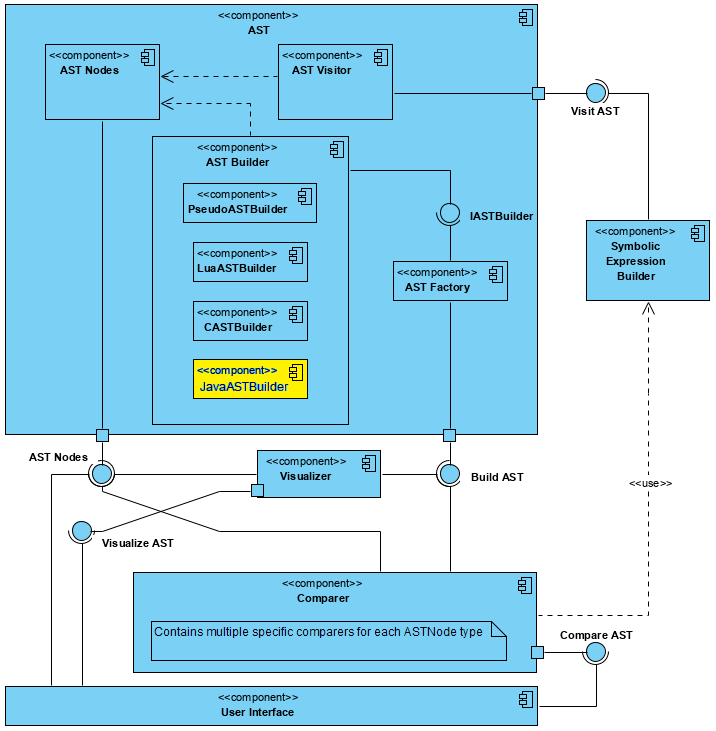
\includegraphics[width=\textwidth]{UML_with_Java_builder_added.png}
\caption{UML diagram of LINVAST implementation with new component added (Java builder)}
\label{fig:UML}
\end{figure}

Builder should extend \texttt{ANTLR\_GENERATED\_BASE\_VISITOR<ASTNode>} in order to implement methods for recursive visit of ANTLR parse tree (a visitor method for every ANTLR tree node type). These methods return language invariant AST nodes, and when whole parse tree is visited, the whole AST is created and returned.

In Figure \ref{fig:example} there is an example of difficulty we faced. There is a discrepancy between Java parse tree and the AST. First two images of the figure show that Java uses two node types to represent variable declaration: modifier (e.g. public, private, static, final, etc.) and fieldDeclaration (e.g. <type> <var> = <expression>, int x = 3). On the other hand, the AST separates variable declaration bit differently: Declaration Specifier Node type stores both modifiers and type name, and declarator stores the rest (e.g. x = 3). Hence there is no trivial mapping between Java parse tree node types and AST node types.


\begin{figure}[H]
\begin{lstlisting}
classBodyDeclaration
    : ';'
    | STATIC? block
    | /\colorbox{lightblue}{modifier*}/ memberDeclaration
    ;
    
memberDeclaration
    : methodDeclaration
    | genericMethodDeclaration
    | /\colorbox{lightgrey}{fieldDeclaration}/
    | constructorDeclaration
    | genericConstructorDeclaration
    | interfaceDeclaration
    | annotationTypeDeclaration
    | classDeclaration
    | enumDeclaration
    ;
\end{lstlisting}

\begin{lstlisting}
fieldDeclaration
    : / \colorbox{lightblue}{typeType}/ variableDeclarators ';'
    ;
    
variableDeclarators
    : /\colorbox{lightred}{variableDeclarator}/ (',' /\colorbox{lightred}{variableDeclarator}/)*
    ;

/\colorbox{lightred}{variableDeclarator}/
    : /\colorbox{yelloworange}{variableDeclaratorId}/ ('=' /\colorbox{green}{variableInitializer}/)?
    ;
    
\end{lstlisting}

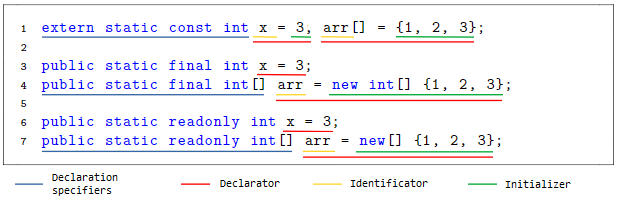
\includegraphics[width=\textwidth]{declaration_decomposition_v2.png}
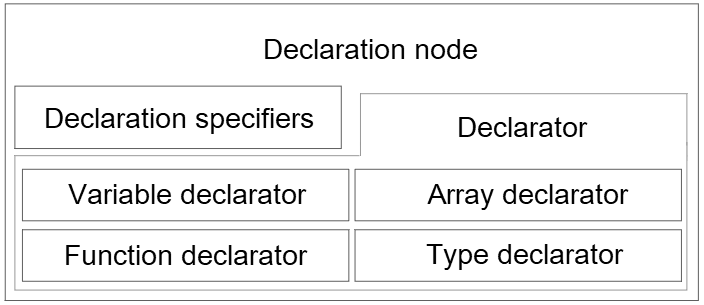
\includegraphics[width=\textwidth]{declaration_nodes_v4.png}

\caption{Example of discrepancy between ANTLR parse tree and the language invariant AST}
\label{fig:example}
\end{figure}

\section{Examples of Language-invariant AST generated from Java source}
\label{sec:examples}

Since not all visitor methods have been implemented yet, the examples are small, e.g. for now we can only show examples with empty block statements.

\begin{figure}[h!]
\begin{center}
\begin{lstlisting}
public class HelloWorld{

}
\end{lstlisting}

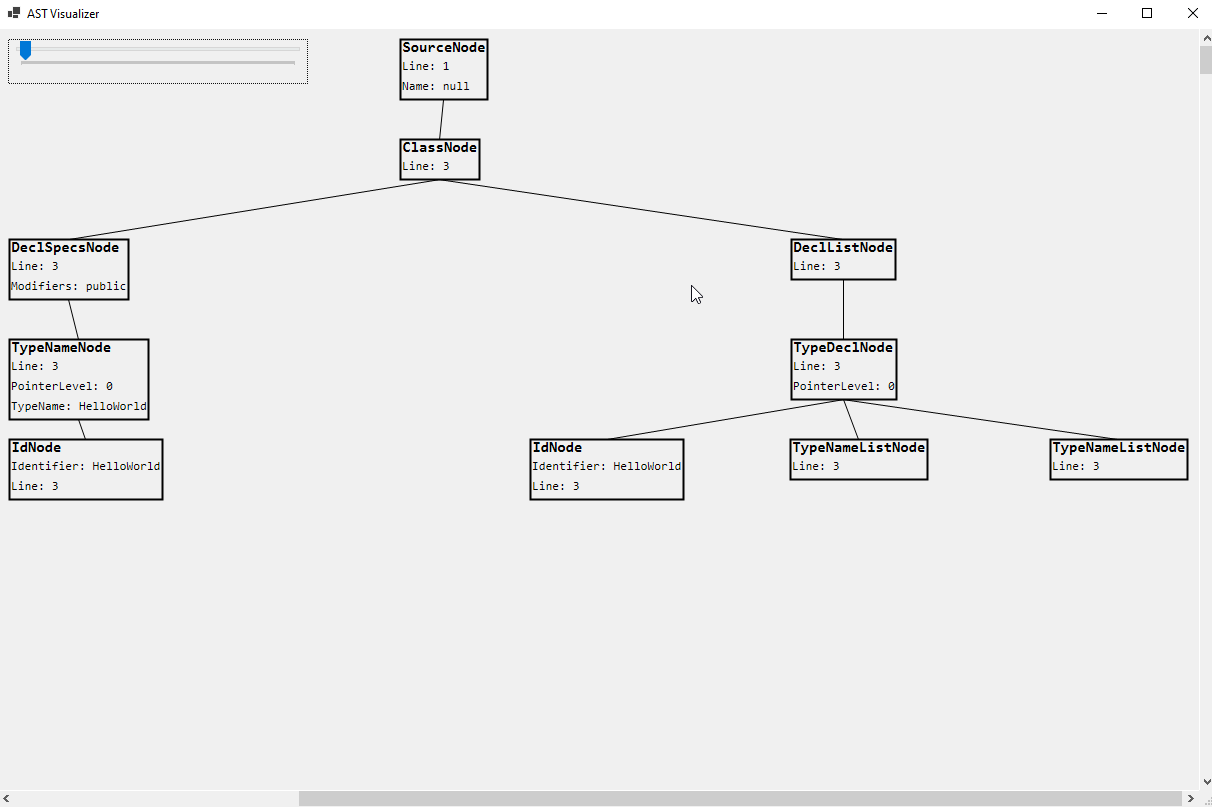
\includegraphics[width=\textwidth]{ast}
\caption{Empty class \textbf{HelloWorld}}
\label{fig:ast1}
\end{center}
\end{figure}

\begin{figure}[h!]
\begin{center}
\begin{lstlisting}
public class Animal {

	public String name;
	
	public void eats();
}
\end{lstlisting}
Image of AST will be added here.\\
     \centering
     \begin{subfigure}[b]{\textwidth}
         \centering
         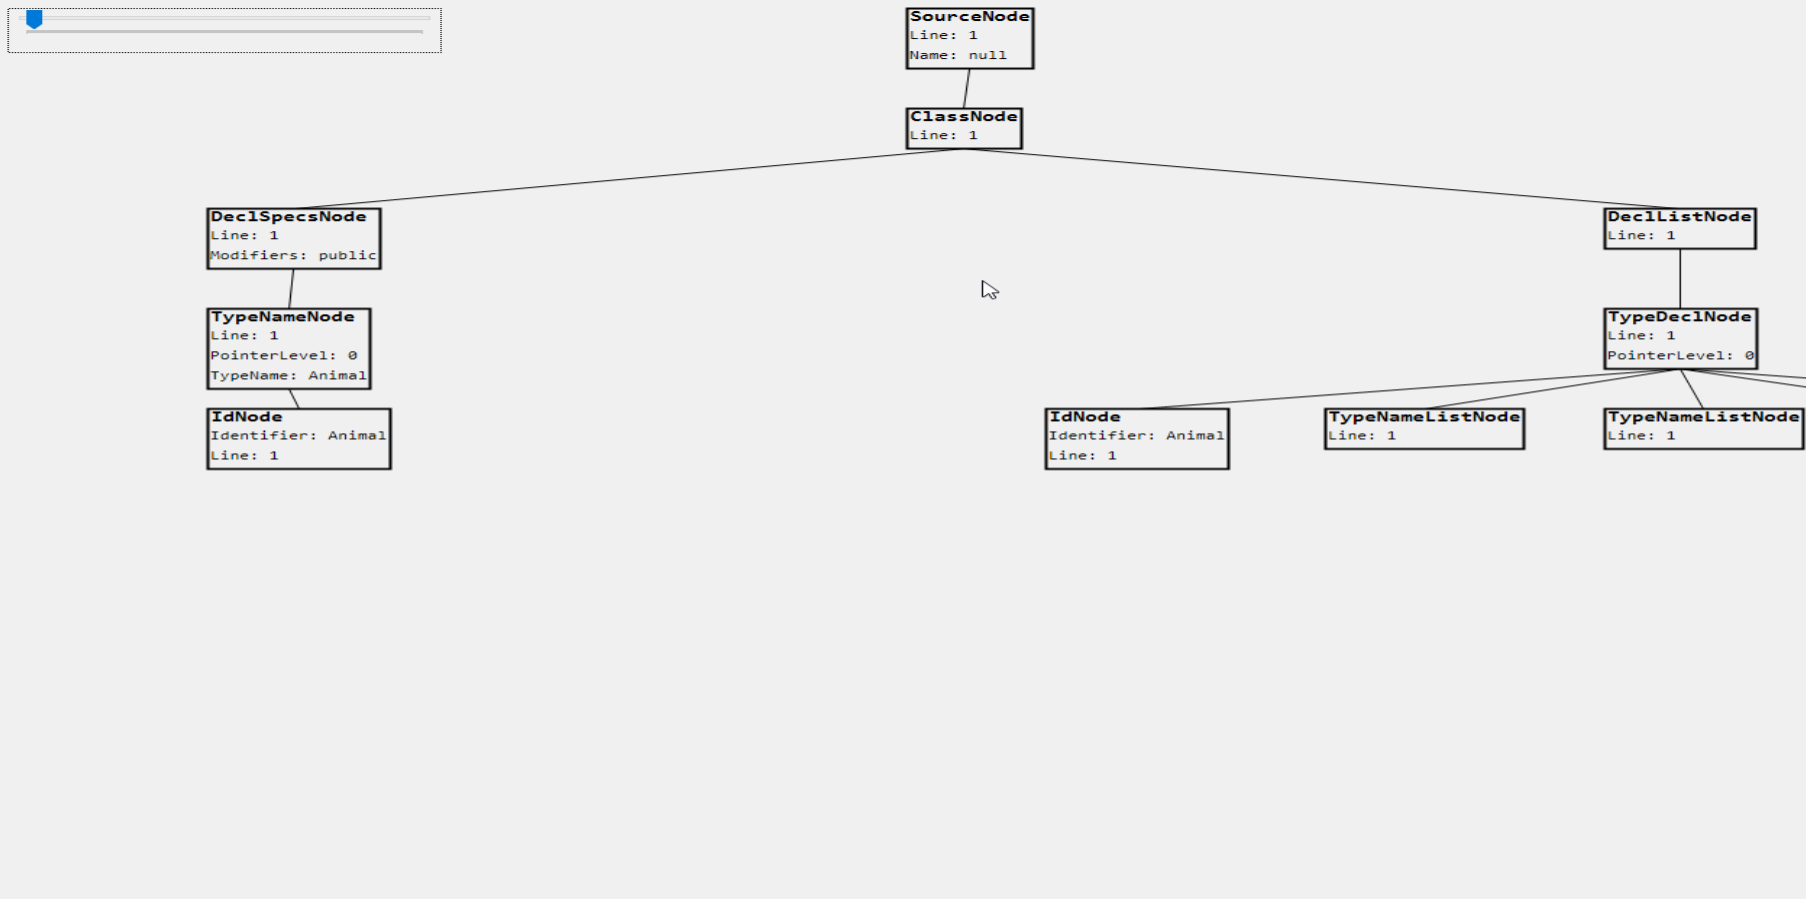
\includegraphics[width=\textwidth]{animal_ast1}
         \caption{First part of the tree}
     \end{subfigure}
     \quad
     \begin{subfigure}[b]{\textwidth}
         \centering
         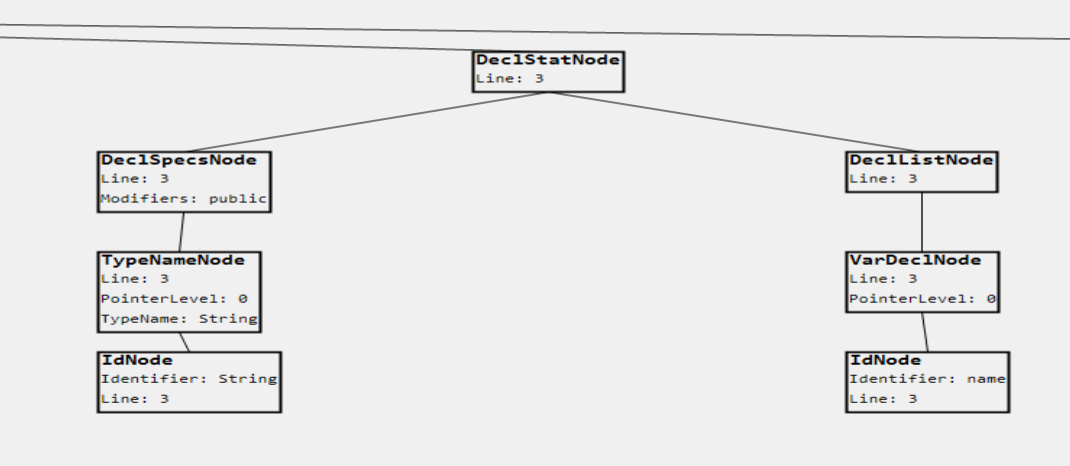
\includegraphics[width=\textwidth]{animal_ast2}
         \caption{Second part of the tree}
     \end{subfigure}
     \begin{subfigure}[b]{\textwidth}
         \centering
         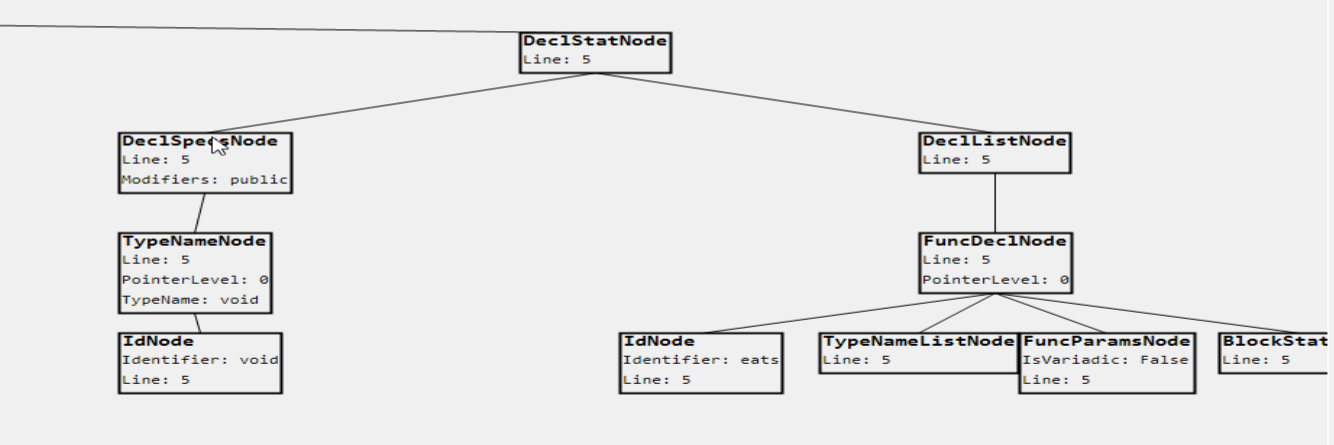
\includegraphics[width=\textwidth]{animal_ast3}
         \caption{Third part of the tree}
     \end{subfigure}

%\includegraphics[width=\textwidth]{}
\caption{\textbf{Animal} class example}
\label{fig:ast3}
\end{center}
\end{figure}


\begin{figure}[h!]
\begin{center}
\begin{lstlisting}
public class Rabbit extends Animal {

	public void eats(){
		System.out.println("Rabbits eat carrots.");	
	}
}
\end{lstlisting}
Image of AST will be added here.\\
     \centering
     \begin{subfigure}[b]{\textwidth}
         \centering
         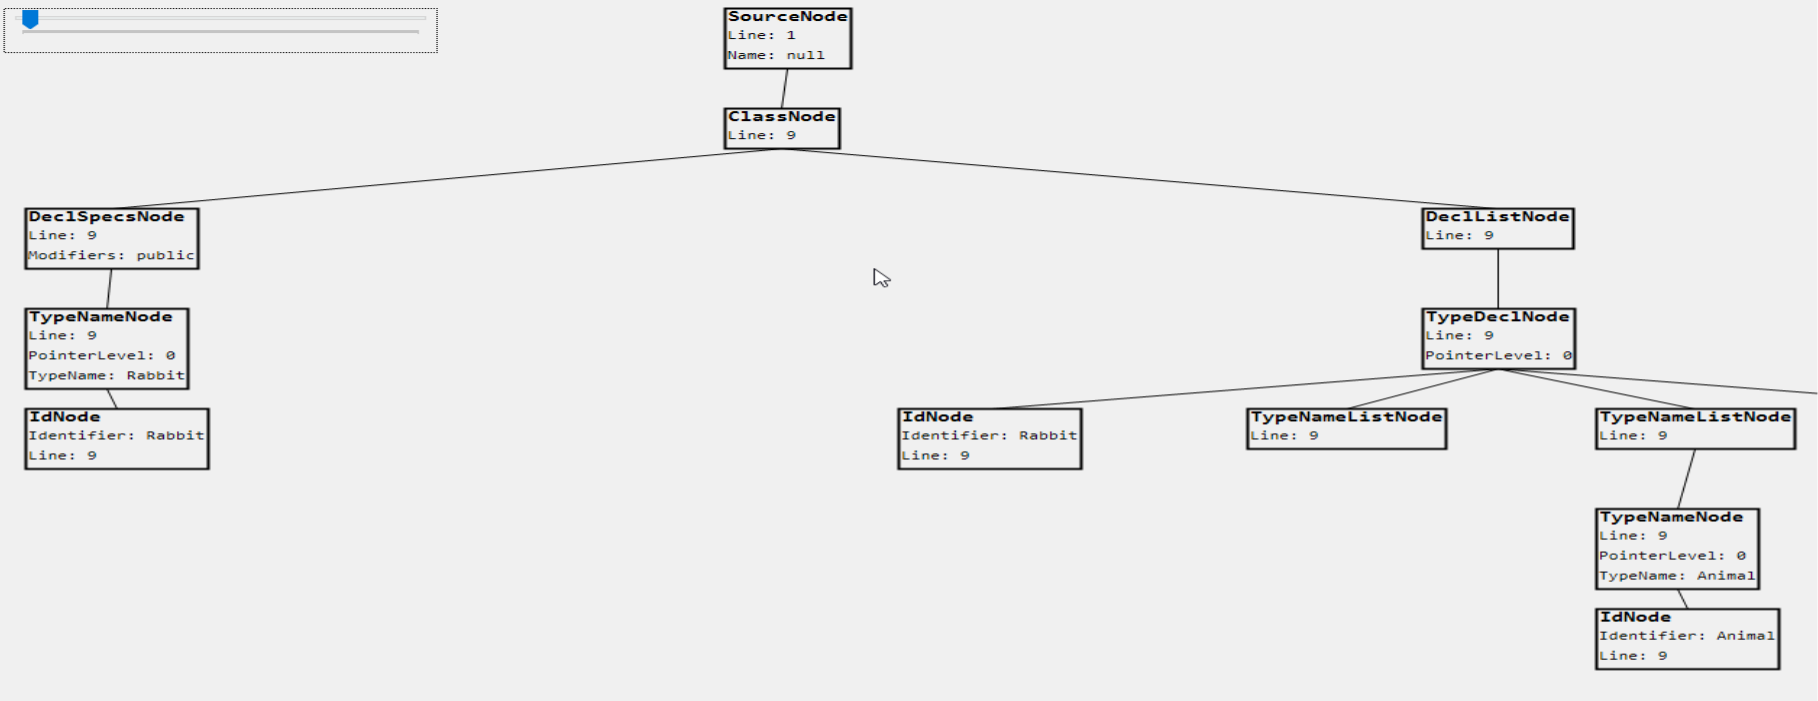
\includegraphics[width=\textwidth]{rabbit_ast1}
         \caption{First half of the tree}
     \end{subfigure}
     \quad
     \begin{subfigure}[b]{\textwidth}
         \centering
         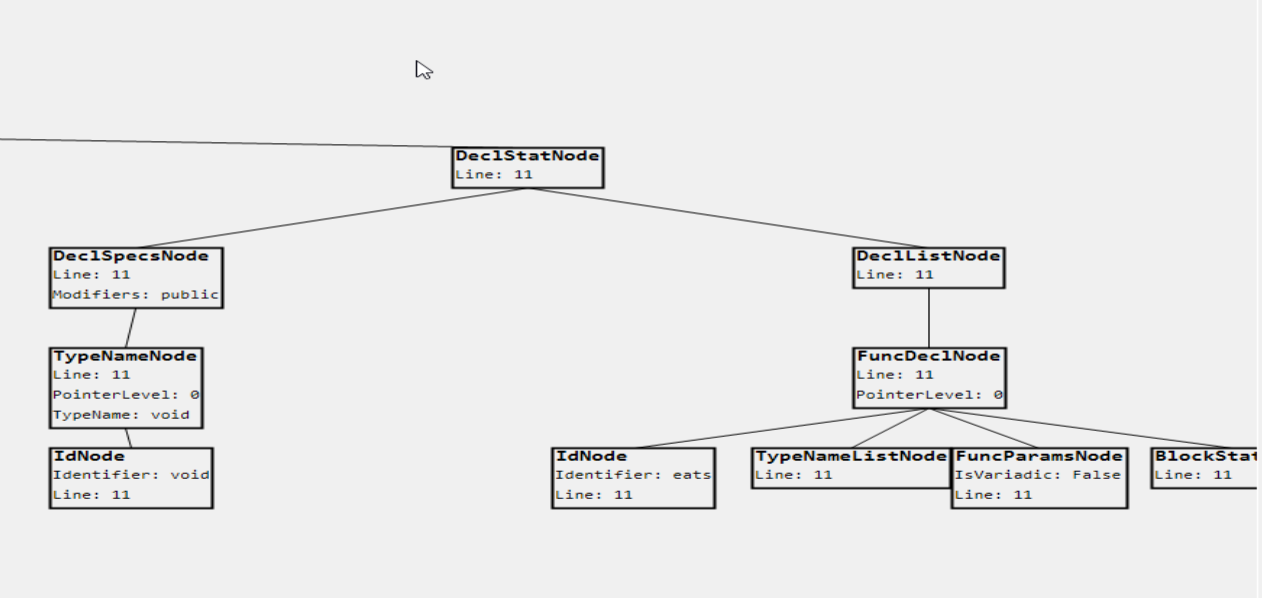
\includegraphics[width=\textwidth]{rabbit_ast2}
         \caption{Second half of the tree}
     \end{subfigure}

%\includegraphics[width=\textwidth]{}
\caption{Example with parent class}
\label{fig:ast3}
\end{center}
\end{figure}


\end{document}
